%********** Chapter 4 **********
\chapter{Electronic Pet}\index{Electronic Pet}\index{projects!Electronic Pet}\label{ch:pet}

\section{Introduction}

This chapter introduces the third project: the Electronic Pet.  The Electronic Pet program is similar to Tamagotchis, little electronic toy ``pets'' that have buttons to feed them, play with them, etc.  As with the previous projects, the initial version is limited, a pet can only be named, fed, and played with.  However, the structure of the program is flexible, making it relatively simple to add more features to the pet.  

This project reviews the topics covered in Chapters 2 and 3 and introduces several new elements of programming:
\begin{tight_itemize}
\item Classes\index{classes}, including:
\begin{tight_itemize}
\item Objects
\item Data members
\item Member functions (methods)
\item Constructors
\item Public and Private
\end{tight_itemize}
\item Strings\index{strings} 
\item Files\index{files}
\end{tight_itemize}

 A class is an abstract definition of a \emph{data structure}\index{data structure} that stores data and has functions that can act on the data.  Once a class is defined the programmer can create \emph{objects}\index{object} whose type is the same as the class.  For example, in this project, a \codefont{pet} class is defined and an object of type \cf{pet} is created.  A string is a new data type that can hold a ``string'' of characters.  It is useful for storing names, addresses, and similar types of data.  Files are used to store data when a program isn't running and to share data between programs.  In C++ the syntax for reading from and writing to files is similar to the syntax for reading from and writing to the keyboard and screen.

%\begin{itemize}
 % \item Classes
 % \item Data members
 % \item Function members
 % \item Constructors
 % \item Public versus private
 % \item Strings
%\end{itemize}

\section{The Program}

Listings~\ref{listing:electronic pet} and~\ref{listing:pet class} present the code for an electronic pet.  The program is divided into two sections.  Enter the code from \emph{both} Listings~\ref{listing:electronic pet} and~\ref{listing:pet class} as one long program, starting with the code in Listing~\ref{listing:electronic pet}.  (Again, do not enter the line numbers.)  As the program is entered, try to figure out what the statements do.  Many of them should be familiar, but others will be new.

\begin{minipage}{\textwidth}
\begin{lstlisting}[language=C++,numbers = left, xleftmargin=4.0ex, basicstyle=\small,emph={hunger, happy,name,pet1,choice,health_check},emphstyle = \color{\mycolor},
showstringspaces=false,
caption = {The \codefont{main()} and the declaration of the \cf{pet} class.},
label={listing:electronic pet}]
#include<iostream>
#include<string>
using namespace std;
// declaration of the pet class
class pet{
   private:
      int hunger;           // private data member
      int happy;            // private data member
      string name;          // private data member
   public:
      pet();                // constructor
      void play();          // public member function
      void feed();          // public member function
      void print();         // public member function
      int check_health();   // public member function
};
int main()
{
   pet pet1;
   int choice;
   int health_check;
   do{
       pet1.print();
       cout << "What would you like to do with your pet?\n";
       cout << " Play (1) \n Feed (2) \n Exit (0) \n";
       cin >> choice;
       switch(choice){
       case 1:
           pet1.play();
           break;
       case 2:
           pet1.feed();
           break;
      }
      health_check = pet1.check_health();
   }while(choice != 0 && health_check != 1);
   cin.ignore();
   cout << "Press enter to exit." << endl;
   cin.ignore();
   return 0;
}
\end{lstlisting}
\end{minipage}

Once the entire program has been entered, compile it.  As always, there may be some copying errors that need to be fixed.  Once the program compiles, run it and see what it does.  Be sure to test all of the menu options.  Are there any choices that produce unexpected output?  What happens if a nonexistent menu option is tried?  How do the user's choices affect a pet?

As with the previous projects, this program has some shortcomings.  Most notably, there are a limited number of options.  However, the program is written to make it easy to add to the pet's behavior, making it more fun and interesting to play with.  


\begin{minipage}{\textwidth}
\renewcommand*\thelstnumber{\the\value{lstnumber}b}
\begin{lstlisting}[language=C++,numbers = left,xleftmargin=4.0ex, basicstyle=\small, emph={hunger, happy,name,pet1,choice,health_check},emphstyle = \color{\mycolor},
showstringspaces=false,
caption = {Definition of the functions of the \cf{pet} class.},
label={listing:pet class}]
/* Constructor, creates a new pet with starting values. */
pet::pet(){
     hunger = 50;
     happy = 50;
     cout << "Pet's name? (One word) ";
     cin >> name;
}
/* Member function play(), allows playing with a pet. */
void pet::play(){
    int choice = 0;
    cout << "What should we play?\n";
    cout << " Fetch (1) \n Roll over (2) \n";
    cin >> choice;
    switch(choice){
    case(1):
         happy += 10;
         hunger += 5;
         break;
    case(2):
         happy += 5;
         hunger += 1;
         break;
    default:
         cout << "Not a valid choice." << endl;
   }
}
/* Member function feed(), allows the user to feed a pet. */
void pet::feed(){
    cout << "\nMMM, Yummy!\n";
    hunger -= 5;
}
/* Member function print(), prints information about a pet. */
void pet::print(){
    cout << "\nYour pet " << name << " is " << endl;
    cout << "Happy: " << happy << endl;
    cout << "Hungry: " << hunger << endl;
}
/* Member function check_health(), checks the health of a pet. */
int pet::check_health(){
    if(hunger >= 100){
         cout << "\nYour pet has starved.\n";
         return 1;
    }
    if(happy <= 0){
         cout << "\nYour pet has died of a broken heart.\n";
         return 1;
    }
    return 0;
}
\end{lstlisting}
\end{minipage}

\subsection{Classes}\index{classes}

 A \emph{class} is an abstract data structure consisting of \emph{data members}\index{data member}\index{classes!data member} and \emph{member functions}\index{function member}\index{classes!function member}, which are also called \emph{methods}\index{methods}\index{classes!methods}.  Data members are elements that store the data for an object\index{object}.  Member functions (or methods) are functions that act on that data.  A class can have multiple data members with different types and multiple member functions.  Figure~\ref{fig:class1} illustrates this idea for the \cf{pet} class used in this project, which has three data members and five member functions.  Once a class is defined, the programmer can create objects whose type is the class.  In this project, a \codefont{pet} class is defined, which allows objects of type \cf{pet} to be created.

A class is basically a programmer-defined, compound type.  Types, (e.g., \codefont{int} and \codefont{double}) allow the programmer to declare variables and to use the variable to store data.  For each type, there are associated operations (e.g., + and -) that can act on the variables.  
A class allows the programmer to declare objects, which can be thought of as variables whose type is a class and which can contain several pieces of data. For example, in this project, \codefont{pet1} is an object of type \codefont{pet} (see line 19), which stores several pieces of data regarding the pet (its hunger, happiness, and name).  Each class has associated functions, the member functions or methods, that can act on an object's data.    

A class definition is typically divided into two parts: the \emph{declaration} of the overall structure of the class (which is somewhat like a function prototype and contains prototypes for all of the class member functions) and the \emph{definitions} of the class member functions.  As with function definitions and prototypes, the class structure must be included before \cf{main()}\footnote{Or, more generally, it must be declared before it is used, just like variables and functions must be declared before they are used in the code.} and then the definitions of the functions (the actual function code) may be included later.  For example, in this project the structure of the \cf{pet} class is declared on lines 6-16, but the definitions of the member functions are defined on lines 1b-49b.\footnote{An alternative approach is to put the class in a separate file, which is discussed in later chapters.}

The data and functions of a class are accessed using \emph{dot notation}\index{dot notation}, which consists of the name of an object followed by a dot (.), followed by the name of the data member or member function to be accessed (see Figure~\ref{fig:memberfunctioncall}).  For example, line 23 shows the object named \codefont{pet1} accessing the \codefont{print()} member function of the \cf{pet} class using the statement:\\
\codefont{pet1.print()};\\
this makes the \codefont{pet1} object call its \codefont{print()} function, which is a member function of the class \codefont{pet}.

\subsection{Strings}\index{strings}\index{libraries!string@{\cf{string}}}

The term \emph{string} is a generic name for any data structure that holds a ``string'' of characters.  In C++ two types of strings are common, string objects and C-style strings.  In this chapter string objects are used, C-style strings are discussed in Interlude 4.   String objects are defined by the \cf{string} class, which is defined in the string library.  The string library is included on line 2 in the program.  Without line 2, the compiler and the program wouldn't know what a string was and any reference to a string in the code would generate a compiler error.  

A \cf{string} object holds a string of characters.  For example, in this program, the \codefont{name} object, which is of type \cf{string}, is used to store the name of the pet.  Strings can be obtained and printed using \codefont{cin} and \codefont{cout} just like other variables (see lines 6b and 34b).  The \cf{string} class contains dozens of member functions that can be used to manipulate, input, and output strings.  Only a few of the most useful functions are covered in this chapter.  Some of the other useful functions in the \cf{string} class are listed in Section~\ref{appendix:string} of Appendix A.

\section{Analysis  of the Code}

This program creates a single object of the \cf{pet} class; that is, it creates a ``pet.''  
%Each pet object has a \codefont{name}, a level of \codefont{happy}, and a level of \codefont{hunger}.  
A menu allows the user to select different ways to interact with the pet.  Each interaction has a different effect on the pet.  
The analysis of the code begins by analyzing the \codefont{pet} class.  Once it is clear how the class works, it's much easier to understand the rest of the program.
  
\mysubsubsection{Lines 5-16: The Pet Class Declaration}

Lines 5-16 declare the \cf{pet} class.  
%  As with function prototypes, a class must be declared before it can be used, typically before the \codefont{main()} function, and the actual code defining the functions of a class can come at the end of the program. 
Once the \cf{pet} class has been declared pet objects can be created (line 19).  Each pet object is a unique object that, like a variable, stores its own data.  Each pet object represents a unique, simulated pet that the user can interact with.  

Figure~\ref{fig:class1} illustrates the members of the \cf{pet} class, showing its three data members and five member functions in one structure.

Line 5 is the beginning of the definition of the \cf{pet} class.  (The rules for naming new classes are exactly the same as for other variables -- any valid variable name is a valid class name.)

Line 6 declares that the next few lines define \emph{private}\index{private} members of the \cf{pet} class.  The meaning of \emph{private} and \emph{public} will be discussed later in the chapter.  Each pet object has the following private data members:
\begin{tight_enumerate}
\item \codefont{hunger} - This is an integer that keeps track of the pet's current hunger level.  Feeding the pet decreases a pet's \codefont{hunger}, and playing with the pet increases it.  If a pet's \codefont{hunger} exceeds 99, the pet starves to death.
\item \codefont{happy} - This is an integer that keeps track of the pet's current happiness.  Playing with the pet increases its happiness.  If a pet's happiness reaches zero, the pet dies of a broken heart, although in the current version of the program happiness can only increase.
\item \codefont{name} - This is a string object that records the pet's name.  The user selects the name.
\end{tight_enumerate}


Line 10 declares that the next few lines define \emph{public}\index{public} members of the pet class.
Lines 11-15 declare the five member functions of the pet class:
\begin{tight_enumerate}
\item \codefont{pet()} - This is a \emph{constructor} for the \cf{pet} class.  It is called whenever a new pet is created.  It sets the pet's initial \codefont{hunger} and \codefont{happy} values and asks the user for the pet's name.
\item \codefont{play()} - This function allows the user to play with the pet.
\item \codefont{feed()} - This function allows the user to feed the pet.
\item \codefont{print()} - This function prints the information about the pet.
\item \codefont{check\_health()} - This function checks the health of the pet.  If the pet's \codefont{hunger} value is too high or its \codefont{happy} value is too low, the function prints a condolence message and returns a value to let the rest of the program know that the pet died.
\end{tight_enumerate}

Each of these member functions can manipulate the data members of a \cf{pet} object (e.g., can modify a pet's hunger, happiness, etc.).  Each of lines 11-15 serves the same role as a function prototype; it tells the compiler what the return type of each function is and what arguments each function should receive.  In this case, only the \codefont{check\_health()} function returns a value (of type \cf{int}); the rest are void.  Member functions can have parameters, although none of these do.  

Thus, the \cf{pet} class creates a new data structure that can store several pieces of data: a pet's name, happiness, and hunger, and defines a number of functions that can manipulate that data.  

\begin{figure}
%\centerline{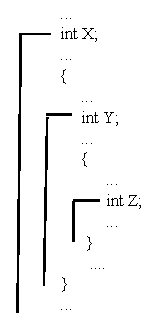
\includegraphics[width=9cm,height=6cm]{images/scope1.eps}}
\setlength{\unitlength}{1cm}
\begin{picture}(8,5)

\linethickness{0.3mm}
\put(1,4.5){\codefont{The Pet Class}}
\put(1.5,4){\codefont{hunger = }}
\put(1.5,3.5){\codefont{happy = }}
\put(1.5,3){\codefont{name = }}
\put(1.5,2.5){\codefont{pet()}}
\put(1.5,2){\codefont{play()}}
\put(1.5,1.5){\codefont{feed()}}
\put(1.5,1){\codefont{print()}}
\put(1.5,0.5){\codefont{check\_health()}}

\put(5.5,3.5){Data members; these store data for the pet objects.}
\put(5.5,1.5){Member functions (or methods);}
\put(5.5,1.0){these functions are used to manipulate the data of pet objects.}

\ifcolor\color{\mycolor}{
\put(1.25,4.4){\line(1,0){4}}
\put(1.25,0.4){\line(1,0){4}}
\put(1.25,4.4){\line(0,-1){4}}
\put(5.25,4.4){\line(0,-1){4}}
\put(1.25,2.9){\line(1,0){4}}
\ifcolor}
\end{picture}
\caption{An illustration of the \cf{pet} class.  Classes contain data members that hold information about objects of the class type (e.g., hold information about pet objects).  Classes also have member functions that act on the data.}
\label{fig:class1}
\end{figure}

\subsection{Lines 1b-49b: Defining the \cf{Pet} Class Member Functions}

Lines 1b-49b define each of the \cf{pet} class's member functions.  Each function definition begins with a line similar to those for functions in Chapter 4, but with the addition of \codefont{pet::} before the function name (lines 2b, 8b, 28b, 33b, and 39b).  This tells the compiler that these functions are part of the \cf{pet} class.  It's legal to have two functions with the same name, one that's a member of the class and one that is not.  The \codefont{pet::} denotes the function that is a member of the class.

\mysubsubsection{Lines 1b-7b: The Constructor}

A constructor\index{constructor} is a special type of member function.  A constructor is called when a new object is created.\footnote{A class can have multiple constructors, if each constructor has a different number or types of parameters.  A constructor with parameters is called like any other function, but when the object is declared.  For example, \codefont{pet pet2(7);} creates a new pet object named \codefont{pet2} using the constructor for the \cf{pet} class that has a single integer as a parameter.  If no such constructor exists, this would produce a compiler error.} A constructor has the same name as the class (e.g., \cf{pet}).  Its return type is predetermined and is not included in the program.  Thus, on line 10 and line 2b, the \codefont{pet()} function has no return type, not even \cf{void}.

On line 19 when the object called \codefont{pet1} of type \cf{pet} is created, the constructor function \codefont{pet()} is automatically called.  The pet constructor sets the new pet object's \codefont{hunger} to 50 (line 3b) and its \codefont{happy} to 50 (line 4b), and asks the user for the new pet object's name (lines 5b-6b).  The $>>$ operator reads in a string of characters up to the first whitespace character (space, tab, newline, etc.) and then stops, which is why the pet can have only one name, not a first and last name.  Later, this limitation will be removed.

Line 1b is a comment explaining what this function does.  As a comment, it does not have any effect on how the program behaves. 

\mysubsubsection{Lines 8b-26b: The \codefont{play()} Function}

This function allows the user to ``play'' with his or her pet.  Using the same basic menu structure as in Chapter 3, the user can choose to either play fetch or roll over with the pet.  Playing fetch makes the pet happier, but also hungrier (lines 16b and 17b), whereas rolling over makes the pet a little happier and only a tiny bit hungrier (lines 20b--21b).  

Note that on these lines, a new operator \codefont{+=} is being used.  The command:\\
\codefont{
happy += 10;\\
}
is equivalent to:\\
\codefont{
happy = happy + 10;\\
}
Both take the current value of the variable \codefont{happy} and add 10 to it.  The \codefont{+=} operator is just a shortcut.  Similar operators (\codefont{-=}, \codefont{*=}, etc.) are listed in Section~\ref{appendix:operators} of Appendix A.

\mysubsubsection{Lines 27b-31b: \codefont{The feed()} Function}

This function allows the user to ``feed'' the pet, thereby decreasing its hunger (here, the \codefont{-=} operator is used).
It also has the pet print some output to the user (line 29b).

\mysubsubsection{Lines 32b-37b: The \codefont{print()} Function}

This function prints information about a pet, its name, and how happy and hungry it is.  

\mysubsubsection{Lines 38b-49b: The \codefont{check\_health()} Function}

% check, has <= been used before?
This function checks the hunger (line 40b) and happiness (line 44b) of the pet.  If the pet is too hungry (hunger is larger than or equal to 100) or too unhappy (happy is less than or equal to 0), then an appropriate message declaring the demise of the pet is printed and the value 1 is returned.  If the pet is not too hungry or too unhappy, the value 0 is returned.  Note the use of the Boolean comparison operators \codefont{$<=$} and \codefont{$>=$} which stand for ``less than or equal to'' and for ``greater than or equal to'' respectively.

The return value is necessary because, in the \codefont{main()} function, the program should behave differently depending on whether the pet is alive or dead.  Currently, if the pet is alive, the program loops back to the beginning and allows the user to continue playing with or feeding the pet (lines 36 and 22), whereas if the pet dies, the program ends.  This could be changed, for example, to having the program ask if the user wants to create a new pet if the current pet dies.

\subsection{Lines 1-3 and 17-50: The Main Program}

Most of Listing~\ref{listing:electronic pet} is taken up with the \codefont{main()} function, which utilizes the \cf{pet} class.

\mysubsubsection{Lines 1-3: \#includes}
As with the previous programs, these lines are preprocessor commands for including additional libraries.  A new library, the string library, is used in this project and is included on line 2.

\mysubsubsection{Lines 19-20: Declaring variables (and objects)}

These lines declare the variables used in the \codefont{main()} function.  Two are integers: \codefont{choice} and \codefont{health\_check}.  These are assigned the values 3 and 0, respectively.  It is a good idea to assign values to variables when they are declared; otherwise, the variables hold a random value, which could cause the program to behave unpredictably.

Line 19 declares an object called \codefont{pet1} of type \cf{pet} -- the new class created for this program.  As noted above, when a new object is created, the constructor for that class is automatically called.  The constructor sets the initial values for \codefont{hungry} and \codefont{happy} for the new pet object and asks the user for a name for the pet (lines 2b-6b).

Once a class has been defined an unlimited number of objects of that type can be created.  So, although currently the program creates only one pet object (called \codefont{pet1}), many more pet objects could be created just as many variables of type \codefont{int} can be created within a program.  Each pet that's created has its own \codefont{hunger}, \codefont{happy}, and \codefont{name}.
To create more pets add a line to \cf{main()} like:\\
\codefont{pet pet2, another\_pet, X;}\\
This will create three more pet objects (with the names \codefont{pet2}, \codefont{another\_pet}, and \codefont{X}).  For each pet object, the constructor will be called, so three more pet names will be requested.  To print or play with one of the new pets, the dot notation is used: \codefont{pet2.print();} or \codefont{X.play();}\\  

\mysubsubsection{Lines 22-36: The Main Loop}

This loop is similar to the ones in both the NIM and Calculator programs.  It allows the program to repeat until either the pet dies or the user loses interest and quits.  These two conditions for ending the program are coded in the while condition on line 36.

Remember that the loop continues so long as the condition is \emph{true}.  So, the condition on line 36 can be read as \emph{while the user didn't choose option 0 (\codefont{choice != 0}) AND (\&\&) the pet is alive (\codefont{health\_check != 1}), loop back to the beginning}.

\begin{figure}
%\centerline{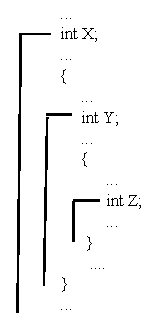
\includegraphics[width=9cm,height=6cm]{images/scope1.eps}}
\setlength{\unitlength}{1cm}
\begin{picture}(13,3)

\linethickness{0.3mm}
\put(6,1.5){\codefont{pet1.print( );}}
\put(5,2.5){object name}

\put(5.7,0.6){dot}

\put(6.1,3){function name}

\put(8,2.5){parentheses (required)}

\put(7.6,0.4){arguments (if any)}

\color{\mycolor}{
\put(5.9,2.4){\vector(1,-1){0.5}}
\put(6.2,0.9){\vector(1,1){0.5}}
\put(7.3,2.9){\vector(0,-1){1}}
\put(9.2,2.4){\vector(-2,-1){1}}
\put(8.8,0.9){\vector(-1,1){0.5}}
}

\end{picture}
\caption{The dot notation is used to call a member function of a class.}
\label{fig:memberfunctioncall}
\end{figure}

\mysubsubsection{Line 23: Printing the pet}

Line 23 calls the \codefont{print()} function of the class \cf{pet} \emph{specifically} for the object \codefont{pet1}.  Pay close attention to the general syntax of this command, which is illustrated in Figure~\ref{fig:memberfunctioncall}.  First, the name of the object is used (\cf{pet1}), then a dot (period), then the name of the function to be called (\cf{print()}).  Because this is a function, it must be followed by parentheses.  Finally, if the function expects any arguments, they are placed within the parentheses just as for other function calls.
This causes the \cf{pet} object \cf{pet1} to ``print itself,'' specifically, \cf{pet1}'s name, hunger, and happiness.  If there were a second pet object (e.g., a \cf{pet2}) it could also be asked to print itself and it would print its own values.  

\mysubsubsection{Lines 24-34: The Menu}

Lines 24-34 code a menu that allows the user to choose whether to play with or feed the pet.  First the user is prompted to enter a value (lines 24 and 25), then their choice is input (line 26), finally a switch statement is used to take the appropriate action (lines 27-34).  

If the user chooses to play with the pet (option 1) the program calls the \codefont{play()} member function using the dot notation.  If the user chooses to feed the pet (option 2) then the program calls the \codefont{feed()} member function.  
If the user enters a 0, nothing happens in the switch statement because there is no 0 case.  However, \codefont{choice} is assigned the value \codefont{0}, thus when the program reaches line 36, the program exits the main loop.

Finally, if the user enters any number other than 0, 1, or 2, nothing happens in the switch statement because there is no matching case and no default case.  When the program reaches line 36, it jumps back to the beginning of the loop because the choice is not equal to 0.  Output telling the user that he or she made an undefined choice would be helpful; adding it is one of the suggested changes.

\mysubsubsection{Line 35: Health Check}
On line 35, the program calls the \codefont{check\_health()} member function for the object \codefont{pet1}.  This function call is like the others in the program (e.g., lines 23, 29, and 32) except that the \codefont{check\_health()} member function returns a value, which is stored in the variable \codefont{health\_check} for use in the while condition on line 36.

\mysubsubsection{Lines 37-40: Graceful Exit}

Lines 37-40 use the same code as NIM to pause the program before it exits.  This is necessary in environments where the program is run in its own window, which closes as soon as the program ends.

\subsection{Public and Private}\index{public}\index{private}\index{classes!private}\index{classes!public}

The data members and member functions of a class can be either \emph{public} or \emph{private}.\footnote{There are other categories, like \emph{protected}, but they are for more advanced applications and are not covered in this text.} The public data and function members of an object can be accessed from anywhere in the code (if the object is in scope) using the dot notation.  Private members can be accessed only by other members of the class.  For example, in \cf{main()} the public \codefont{play()} member function of the \codefont{pet1} object is legally accessed on line 29.  In contrast, the private \codefont{hunger} data member is accessed (and changed) within the \codefont{play()}, \codefont{feed()}, and \codefont{print()} member functions, but it cannot be accessed directly in \codefont{main()} because \codefont{hunger} is a \emph{private} member of the \cf{pet} class.
  
To see how public and private work, add the following line to the \codefont{main()} function after line 34:\\
\codefont{pet1.hunger = pet1.hunger + 1;}\\
When this program is compiled, the compiler should produce an error message like:\\
\codefont{cannot access private member declared in class `pet'}\\
To avoid this error, the \codefont{hunger} data member can be moved from line 7 to line 11, putting it in the public declarations of the \cf{pet} class and thereby making it a public data member accessible from \codefont{main()}.  With that change, the new program should compile successfully.  

Member functions of a class can also be private.  Try moving line 14 (the declaration of the \codefont{print()} member function)  to line 8, thereby making it private.  When this program is compiled, it should also produce a compiler error like:\\
\codefont{cannot access private member declared in class `pet'}.

Change the pet program back, making \codefont{hunger} private and the \codefont{print()} member function public again.

Public and private allow the programmer of a class to control how objects of that class are used and, simplifies the work of other programmers using the class.  As an example, consider the \codefont{string} object that stores a pet's name.  In creating the \codefont{pet} class, we don't have to consider what the \codefont{string} class is doing, or how it's storing data.  So long as the functions of the class are available for review (which they are, online) and work correctly, the internal details of the class shouldn't matter.  The linking of data and functions, combined with hiding the data and accessing it only through functions, is often referred to as \emph{encapsulation}\index{encapsulation} or \emph{information hiding}\index{information hiding}.  

Encapsulation is useful because it leads to \emph{modularity}\index{modularity} -- the ability to build a complex program from code \emph{modules}\index{modules}.  Again, the \codefont{string} class is a good example.  Since its creation, the \codefont{string} class has probably been used in millions of programs by programmers who don't know what's ``inside'' the class and don't need to know, so long as its member functions work correctly.  Large software projects are often built following a similar modular process: one or more teams program the base classes, and other teams work on writing the full program using those classes as the building blocks.   
This approach to programming, using classes and objects to build a program modularly, is a form of \emph{object-oriented programming}\index{object-oriented programming (OOP)} (\emph{OOP}\index{OOP}) and is one of the dominant programming paradigms in use today.

In general, it is a good idea to make the data members of a class private.  This makes it very difficult for someone using the class to accidentally set a bad value (e.g., setting a pet's happiness to -1000 or putting a zero in the denominator of a fraction class) because the public member functions that are used to access the data can check the values before they are set and make sure they make sense.   The member functions of a class are generally public to give access to the class data members, but classes often include private functions that can be called only by other members of the class.  The project in Chapter 7 includes a class with several private member functions.


\vspace{+0.25cm}
{\color{\mycolor}\noindent\hrulefill}
\section{Exercises: Modifying the Program}

The current Electronic Pet program is not particularly complex.  There are a few menu options and a pet's hunger and happiness levels vary, but there's not much to hold a user's interest for more than a few minutes.  However, the code contains the basic framework for a much more interesting program. 

\mysubsubsection{Exercise 1: The Main Menu}

There are a number of places where the output should be improved.  
In the switch statement in the member function \codefont{play()}, there is a default case (line 24b) that tells the user when he or she has made an invalid choice.  Add a similar default case to the switch statement in the main program (e.g., after line 33) to warn the user if they make an invalid selection.  Also add a \codefont{case 0} for when the user chooses to exit the program.  In general, it's a good idea to have a case for every expected option, even if the case doesn't do anything in the current program.  Additionally, when the default case is added, the \codefont{0} case will incorrectly jump to it, unless there is a separate case for when the user enters a \codefont{0}.

\mysubsubsection{Exercise 2: More Interactive Pets}

When the user chooses to feed the pet he or she gets a message in response: ``MMM, Yummy!'' (line 24b), which makes the program more interactive.  But no such message occurs when the user plays with the pet.  Add similar messages to the \codefont{play()} member function.  Placing them within the switch statement (e.g., after lines 17b and 21b), allows different messages depending on the user's choice.  

\mysubsubsection{Exercise 3: More Interesting Output}

Modify the \codefont{print()} member function to give more interesting output.  Instead of simply printing the values of \cf{happy} and \cf{hungry}, use an \codefont{if} statement to print messages that are more appropriate to the pet's level of happiness and hunger.  For example, adding:\\
\codefont{
if(hungry > 80 \&\& hungry < 90)\{\\
\hspace*{0.5cm} cout $<<$ "I'm starving!  Feed me!\textbackslash n";\\
\}\\
}
to the \codefont{print()} member function will make the pet ``respond'' based on its \cf{hunger} level.  Use a series of similar conditionals for different values of \codefont{hungry} and \codefont{happy} to create more interesting output.

\mysubsubsection{Exercise 4: Randomized Output}

The \codefont{feed()} member function always prints the same message every time the pet is fed.  Use a random number and a switch statement to make the pet print a variety of messages when it is fed.  

\mysubsubsection{Exercise 5: More Play Options}

When a user chooses to play with the pet he or she only has two options: to play fetch or roll over.  Expand the number of cases in the switch statement (lines 14b-25b) to give the user more ways to play with the pet.  (Don't forget to include any new options in the output on line 12b.)

\mysubsubsection{Exercise 6: More Feed Options}

Currently, there's only one action associated with feeding the pet; hunger decreases by 5.  Modify the \codefont{feed()} member function to give the user different options for feeding the pet (like the \codefont{play()} member function, which gives the user a several ways to play with a pet).  For example, options could include feeding the pet generic food that decreases hunger, but also decreases happiness; or regular food that only decreases hunger; or fancy food that decreases hunger and increases happiness.  To make this change, add a switch statement, like the one on the \codefont{play()} member function, to the \codefont{feed()} member function.

\mysubsubsection{Exercise 7: Longer Pet Names}

Currently, a pet's name can only consist of a single word (e.g., ``Bob'' or ``Fluffy'').  This is because the input operator $>>$ reads characters only up to the next whitespace.  If the user enters a name like ``Bob P. Fluffles,'' only the ``Bob'' is read -- the rest of the name remains in the input buffer and causes problems later in the program.  The \codefont{string} class has a number of functions that can solve this problem.  The simplest is \codefont{getline(istream, string)} which reads a string of characters up to a newline character (`\textbackslash n') from the \codefont{istream} argument and stores them in the \codefont{string} argument.  Use this function to allow pets to have longer, multipart, names.  (An alternative approach would be to declare several new data members as part of the pet class: \codefont{first\_name}, \codefont{last\_name}, etc.  But it's trickier to get this to work smoothly if the pet's name has a variable numbers of parts: first, last, middle, title, etc.)

\mysubsubsection{Exercise 8: Give Pets a Species}

Add a new data member that stores the type or species of the pet.   The new data member should be of type \codefont{string} like the \codefont{name} data member.  The new data member should be added around lines 7-9, where the other data members are declared.  In addition, the user will need to enter the type of the pet as part of the constructor member function (lines 2b-7b) and the \codefont{print()} member function should print each pet's type (around line 34b).

\mysubsubsection{Exercise 9: Other Pet Qualities}

Expand the \cf{pet} class with at least one additional data member that defines another aspect of the pet's well-being.  For example,  a health data member or a tiredness data member.  Add the data member to the class definition (around line 9), set the initial value as part of the constructor (around line 4b), and make sure the new data member is printed in the \codefont{print()} member function (around line 34b).  Modify the existing member functions to affect the new data member; for example, playing fetch makes a pet healthier \emph{and} more tired.

Add a new member function to manipulate the new data member.  For example, a \codefont{rest()} member function to make the pet less tired, or a \codefont{vet\_visit()} member function to make the pet healthier (and probably less happy).  Include the new member function as part of the class definition (around line 15) and the code for the new function (probably after line 49b, although as a new function, it could be placed anywhere after \codefont{main()}).  A simple way to create new member functions is to copy an existing member function and then modify it, starting by changing the function's name, and then its code.  Add a new option to the main menu to allow the player to choose the new function.

\mysubsubsection{Exercise 10: More Pets}

Add another pet for the user to interact with. 
It is simple to create more than one pet object by adding more pet declarations; for example, \codefont{pet second\_pet;} which creates another pet object named \codefont{second\_pet}.   
Interacting with a second pet object requires statements like: \codefont{second\_pet.play();} and
\cf{second\_pet.feed();}.  
One approach is to copy the switch statement (lines 23 to line 36), then change the pet variable in the second copy, so the user can interact with both of them.  Another approach is to have the program ask the user which pet they want to play with and then use a conditional on the user's choice to select which pet calls the member function.  Something like:\\
\cf{
if(pet\_choice == 1)\{\\
\hspace*{2cm}pet1.play();\\
\}\\
else if(pet\_choice == 2)\{\\
\hspace*{2cm} pet2.play();\\
\}\\
}
Additional changes are required to handle the case where one pet dies and not the other.  (One approach would be an if statement that only allows the user to interact with a pet object only if it passes a health check.)  The next two chapters will introduce data structures that will make it easier to have multiple pets.

\section{Files}\index{files}
\index{close()@{\cf{close()}}}\index{files!close()@{\cf{close()}}}
\index{write}\index{files!write}
\index{read}\index{files!read}

A clear weakness of the Electronic Pet program is that the user can play with a pet only once.  As soon as the program ends, the pet is lost.  This problem can be fixed by using a \emph{file} to store the information about a pet when the program is not running.  In C++, files are accessed using \codefont{fstream} objects (short for \emph{f}ile \emph{stream}).  Typically, an \codefont{ifstream} object (short for \emph{i}nput \emph{f}ile \emph{stream}) is used to read from a file and  an \codefont{ofstream} object  (short for \emph{o}utput \emph{f}ile \emph{stream}) is used for writing to a file. 
File stream objects must open a file before they can send or receive data.  After a file is opened, the program can write to it or read from it using the same operations as are used with \codefont{cin} and \codefont{cout} (e.g., $<<$ and $>>$).  After a program is done using a file, it should close the file.  For example, the code\\
\codefont{
ofstream outfile;\hspace{4cm}\emph{\textbackslash\textbackslash create an ofstream object}\\
outfile.open("filename");\hspace{2.3cm}\emph{\textbackslash\textbackslash Open the file ``filename''}\\
outfile $<<$ "Some text" $<<$ endl; \hspace{0.6cm}\emph{\textbackslash\textbackslash Write some text}\\
outfile.close(); \hspace{4cm}\emph{\textbackslash\textbackslash Close the file}\\
}
opens\index{open()@{\cf{open()}}}\index{files!open()@{\cf{open()}}} a file called ``filename'' for output, writes the string ``Some text'' followed by a new line to the file, and then closes the file.  A similar process is used to open a file to read from it.  For example, the code:\\  
\codefont{
ifstream infile;\hspace{4cm}\emph{\textbackslash\textbackslash create an ifstream object}\\
int x; \\
infile.open("filename");\hspace{2.1cm}\emph{\textbackslash\textbackslash Open the file ``filename''}\\
infile $>>$ x; \hspace{4.3cm}\emph{\textbackslash\textbackslash Read one integer from the file}\\
infile.close();\hspace{4.1cm}\emph{\textbackslash\textbackslash Close the file}\\
}
opens a file called ``filename'' for input, reads a single integer from the file, and then closes the file.  
Modifiers to the \codefont{open()} function allow a file to be opened for appending or to write over the existing file.  If the program attempts to open a file for output and the file doesn't already exist, the program will attempt to create the file.

\mysubsubsection{Exercise 11: Saving a Pet}

Modify the Electronic Pet program to write a pet's data to a file when the program ends and read a pet's data from a file when the program begins.  
The following changes make this possible.  First, when a new pet object is created, the program needs to ask the user whether to create a brand new pet or to load the data for an existing pet from a file.  If the user wants to load a pet, then the program should ask for the pet's name, create an \codefont{ifstream} object,  use the \codefont{ifstream} object to open the file and read the pet information from the file.  For example,\\
\cf{
cin >> name;\hspace{4cm}\emph{\textbackslash\textbackslash get the pet's name, used as the file name}\\
instream infile;\hspace{3.2cm}\emph{\textbackslash\textbackslash create the infile object}\\
infile.open(name.c\_str());\hspace{1.25cm}\emph{\textbackslash\textbackslash open the file\footnote{The \cf{open()} function expects a C-style string (see Interlude 4) not a string object; the \cf{c\_str()} function returns the correct type to the \cf{open()} function.}}\\
infile >> hunger;\hspace{3.1cm}\emph{\textbackslash\textbackslash read the pet's data}\\
... \\
infile.close();\hspace{3.6cm}\emph{\textbackslash\textbackslash close the file}\\
}
Similarly, when the program ends, it should save the data, by creating an \codefont{ofstream} object, opening a file, and writing the pet's data to the file.  Make sure that the data is written to the file in the same order that it is read from the file, otherwise the values of \cf{hunger} and \cf{happy} (for example) may end up switched every time the program is run.

This example uses the pet's name as the file name.  Alternatively the program could ask the user for a file name.

There is one tricky part to opening files.  The file \codefont{open()} function expects the name of the file as a C-style string (covered in Interlude 5), not a \codefont{string} object. If the file name is stored as a \codefont{string}, then a member function of the string class named \codefont{c\_str()} must be used to get the file's name in the right format.  For example:\\
\codefont{infile.open(filename.c\_str());\\}
where \codefont{infile} is an object of type \codefont{ifstream} and \codefont{filename} is an object of type \codefont{string}.

The stream classes include a number of member functions that are useful for accessing data in files, checking whether a file opened correctly, etc.  A few of the most common functions are listed in Section~\ref{appendix:iostream} of Appendix A.

\section{Problems}
It's important to remember that classes are a general way to define any type of object, not just pets.  The programmer can include many different data members or member functions in a class.  This makes classes almost infinitely flexible.  
\begin{enumerate}

\item {\bf Pet Game}\\
 The Electronic Pet program can be turned into a ``real'' game by making it more challenging to balance the pet's different needs.  Add new pet qualities, like health and tiredness, as discussed previously (Exercise 9).  Modify the behaviors so that each user choice increases some values, but lowers others (e.g., playing increases happiness, but also increases hunger and tiredness) so that keeping a pet healthy and happy is a balancing act.

\item {\bf Random Outcomes}\\ 
Currently, the outcomes of user choices are fixed; feed the pet and \codefont{hunger} goes down by a fixed amount (although the user, not having read the code, might not know by how much).  Instead (partially) randomize the outcomes.  For example, feeding a pet lowers \codefont{hunger} by a random amount, and may, in rare cases, make the pet less healthy (e.g., the user got some bad pet food).  Put in appropriate output so the user knows what is happening.  These changes should make the pet game more challenging to play.

\item {\bf Pet Game with Money}\\
To make the pet game even more interesting, add money as a pet quality.  Add options like working or entering competitions, that allow the pet to earn money.  Make actions like buying pet food or toys, or going to the vet, cost money.  

\item {\bf Random Events }\\ Add random events to the program so that every time the user finishes an action, there's a chance that a random event occurs that affects the status of the pet.  This requires a new member function that is called once per loop (like the \codefont{print()} member function).  The function should use at least two random numbers, one to determine if an event occurs and one to determine what event occurs. Example events might include the pet getting injured (lowers health and happiness) or rescuing little Timmy (increases happiness).\footnote{One of the first widely successful video games, The Oregon Trail\texttrademark, originally released in 1974, was based on the same framework of selecting actions to balance resources combined with randomized impacts and events.  Versions of The Oregon Trail continue to be released, and resource balancing in one form or another is an important aspect of many computer games.}

\item {\bf Names in NIM}\\
Change the NIM project so that players can enter their name.  Have the game refer to the player by name instead of saying ``Player 1.''

\item {\bf Files in NIM}\\
Change the NIM project so that it uses a file to keep track of how many times a player has won and lost.  Each time the game starts it should ask the player if they are a new player.  If they are a new player the game should ask them for a new username to store for their record of wins and losses.  If they are a returning player they should enter their previous username and use that to open the correct file.  (Assume that every player will have a unique user name.)  

\item {\bf Spaceship}\\ 
Create a new resource balancing game (for the pet, the resources are happiness, hunger, etc.)  based on flying an interstellar spacecraft to a nearby solar system.  Make the user balance resources like fuel use, oxygen supply, crew happiness, distance traveled, etc.

\item {\bf Planet Game}\\ Create a game that requires balancing the resources of a whole planet (or solar system, universe, multiverse, etc.).

\item {\bf Bank Account}\\ 
A similar structure can be used for nongame applications.  Instead of a \cf{pet} class, create a bank account class with \codefont{checking} and \codefont{savings} as data members.  Instead of play and feed, the user can choose to deposit, withdraw, or transfer to money to savings.  For each action the user will need to input how much money was deposited, withdraw, etc.  The \cf{print()} function should print the current balance in checking and in savings.


%\item Tracking Goals - Very generally, a program with a structure similar to the pet program can be used to track any goal.  For example, the program could be used to track progress towards an A in a course.  Every time the user gets an assignment or a test back they enter it like it was a behavior (instead of feeding their pet, they would finish an assignment) increasing their score/grade.  The program should include positive feedback when the user enters a good score.
\end{enumerate}



